\chapter{Language}\label{ch:language}

\chapquotew{Belittle! What an expression! It may be an elegant one in Virginia, and even perfectly intelligible; but for our part, all we can do is to guess at its meaning. For shame, Mr. Jefferson!}{European Magazine and London Review, 1787\\(reviewing Thomas Jefferson's {\em Notes on the State of Virginia})}{12cm}\index{general}{belittle}

%\topics{what is language, what a language is made of, what properties a language should have for programming computers, how to describe languages}

The most powerful tool we have for communication is language.  This is true whether we are considering communication between two humans, between a human programmer and a computer, or between a network of computers.  In computing, we use language to describe procedures and use machines to turn descriptions of procedures into executing processes.  This chapter is about what language is, how language works, and ways to define languages.

\section{Surface Forms and Meanings}\label{sec:surfaceforms}

A \definition{language} is a set of surface forms\index{general}{surface forms} and meanings, and a mapping between the surface forms and their associated meanings.  In the earliest human languages, the surface forms were sounds but surface forms can be anything that can be perceived by the communicating parties such as drum beats, hand gestures, or pictures.  

%\footnote{Thanks to Charles Yang for this definition.}  
   
A \definition{natural language} is a language spoken by humans, such as English or Swahili.   Natural languages are very complex since they have evolved over many thousands years of individual and cultural interaction.  We focus on \emph{designed} languages that are created by humans for some specific purpose such as for expressing procedures to be executed by computers.

We focus on languages where the surface forms are text.  In a textual language, the surface forms are linear sequences of characters.  A \definition{string} is a sequence of zero or more characters.  Each character is a symbol drawn from a finite set known as an \definition{alphabet}.  For English, the alphabet is the set $\{ a, b, c, \ldots, z \}$ (for the full language, capital letters, numerals, and punctuation symbols are also needed).\sidepicturenocap{0.12}{images/traffic-iStock_000008604065Small}  

A simple communication system can be described using a table of surface forms and their associated meanings.  For example, this table describes a communication system between traffic lights and drivers: 
\begin{center}\vspace*{-1ex}
\begin{tabular}{cc}
\quad Surface Form \quad & Meaning \\ \hline 
\emph{Green} & Go \\
\emph{Yellow} & Caution \\
\emph{Red} & Stop \\ 
\end{tabular}
\end{center}

Communication systems involving humans are notoriously imprecise and subjective.  A driver and a police officer may disagree on the actual meaning of the \emph{Yellow} symbol, and may even disagree on which symbol is being transmitted by the traffic light at a particular time.  Communication systems for computers demand precision: we want to know what our programs will do, so it is important that every step they make is understood precisely and unambiguously.

The method of defining a communication system by listing a table of 
	\[
<\textit{Symbol}, \textit{Meaning}>
\]
pairs can work adequately only for trivial communication systems.  The number of possible meanings that can be expressed is limited by the number of entries in the table.  It is impossible to express any \emph{new} meaning since all meanings must already be listed in the table!
\sidepicturenocap{.3}{images/800px-Marshalite-edit.jpg} % Rotary traffic signal used in Melbourne, Australia}
%http://en.wikipedia.org/wiki/Image:Marshalite_traffic_signal,_Melbourne_Museum.jpg

\shortsection{Languages and Infinity} A useful language must be able to express \emph{infinitely} many different meanings.  \cut{This means the language must contain infinitely many different surface forms.}  Hence, there must be a way to generate new surface forms and guess their meanings (see Exercise~\ref{ex:newforms}).  No finite representation, such as a printed table, can contain all the surface forms and meanings in an infinite language.  
One way to generate infinitely large sets is to use repeating patterns.  For example, most humans would interpret the notation: ``1, 2, 3, \ldots''
as the set of all natural numbers.  We interpret the 	``\ldots'' as meaning keep doing the same thing for ever.  In this case, it means keep adding one to the preceding number. Thus, with only a few numbers and symbols we can describe a set containing infinitely many numbers.  As discussed in Section~\ref{sec:information}, the language of the natural numbers is enough to encode all meanings in any countable set. \cut{(including the set of all possible procedures, as we will see more clearly in Chater~\ref{ch:computability}).}  But, finding a sensible mapping between most meanings and numbers is nearly impossible.  The surface forms do not correspond closely enough to the ideas we want to express to be a useful language.

\cut{
The repeating pattern technique, though, might be sufficient to describe some languages with infinitely many meanings that map onto simple surface forms.  For example, this table defines an infinite language:

\newcolumntype{C}{>{\centering\arraybackslash}p{6cm}}
\newcolumntype{W}{>{\centering\arraybackslash}p{5cm}}

\begin{center}
\begin{tabular}{WC}
{\bf Surface Form} & {\bf Meaning} \\ \hline
\emph{I will run today.} & Today, I will run. \\[0.5ex]
\emph{I will run the day after today.} & One day after today, I will run. \\[0.5ex]
\emph{I will run the day after the day after today.} & Two days after today, I will run. \\[0.5ex]
$\cdots$ & $\cdots$ \\
\end{tabular}
\end{center}

Although we can describe some infinite languages in this way, it is entirely unsatisfactory.\footnote{Languages that can be defined using simple repeating patterns in this way are known as \emph{regular languages}.\LATER{We will define this more precisely in Chapter~[[?]], and see that they are actually a bit more interesting than it seems here.}}  The set of surface forms must be produced by simple repetition.  Although we can express new meanings using this type of language (for example, we can always add one more ``the day after'' to the longest previously produced surface form), the new surface forms and associated meanings are very similar to previously known ones.  
}

\section{Language Construction}\label{sec:language-construction}

To define more expressive infinite languages, we need a richer system for constructing new surface forms and associated meanings.  We need ways to describe languages that allow us to define an infinitely large set of surface forms and meanings with a compact notation.  The approach we use is to define a language by defining a set of rules that produce exactly the set of surface forms in the language.  

\shortsection{Components of Language}A language is composed of:
\begin{itemtight}
\item \emph{primitives} --- the smallest units of meaning.  
\item \emph{means of combination} --- rules for building new language elements by combining simpler ones.
\end{itemtight}

The primitives are the smallest meaningful units (in natural languages these are known as \emph{morphemes}).  A primitive cannot be broken into smaller parts whose meanings can be combined to produce the meaning of the unit.  The means of combination are rules for building words from primitives, and for building phrases and sentences from words.\index{general}{primitive}\index{general}{morpheme}\index{general}{means of combination}

Since we have rules for producing new words not all words are primitives.  For example, we can create a new word by adding \emph{anti-} in front of an existing word.  The meaning of the new word can be inferred as ``against the meaning of the original word''.  Rules like this one mean anyone can invent a new word, and use it in communication in ways that will probably be understood by listeners who have never heard the word before. \cut{There can be no longest English word, since for whatever word you claim to be the longest, I can create a longer one (for example, by adding \emph{anti-} to the beginning of your word).}  

For example, the verb \emph{freeze} means to pass from a liquid state to a solid state; \emph{antifreeze} is a substance designed to prevent freezing.  English speakers who know the meaning of \emph{freeze} and \emph{anti-} could roughly guess the meaning of \emph{antifreeze} even if they have never heard the word before.\footnote{Guessing that it is a verb meaning to pass from the solid to liquid state would also be reasonable.  This shows how imprecise and ambiguous natural languages are; for programming computers, we need the meanings of constructs to be clearly determined.}

Primitives are the smallest units of \emph{meaning}, not based on the surface forms.  Both \emph{anti} and \emph{freeze} are primitive; they cannot be broken into smaller parts with meaning.  We can break \emph{anti-} into two syllables, or four letters, but those sub-components do not have meanings that could be combined to produce the meaning of the primitive.  

\shortsection{Means of Abstraction}In addition to primitives and means of combination, powerful languages have an additional type of component that enables economic communication: \emph{means of abstraction}. \index{general}{means of abstraction}

Means of abstraction allow us to give a simple name to a complex entity.  In English, the means of abstraction are \emph{pronouns} like ``she'', ``it'', and ``they''. The meaning of a pronoun depends on the context in which it is used.  It abstracts a complex meaning with a simple word.  For example, the \emph{it} in the previous sentence abstracts ``the meaning of a pronoun'', but the \emph{it} in the sentence before that one abstracts ``a pronoun''.  

In natural languages, there are a limited number of means of abstraction.  English, in particular, has a very limited set of pronouns for abstracting people.  It has \emph{she} and \emph{he} for abstracting a female or male person, respectively, but no gender-neutral pronouns for abstracting a person of either sex.  The interpretation of what a pronoun abstract in natural languages is often confusing.  For example, it is unclear what the \emph{it} in this sentence refers to.  Languages for programming computers need means of abstraction that are both powerful and unambiguous.

\beforeex
\begin{exercise}\label{ex:newforms}
According to the \emph{Guinness Book of World Records}, the longest word in the English language is \emph{floccinaucinihilipilification}, meaning ``The act or habit of describing or regarding something as worthless''.  This word was reputedly invented by a non-hip\-po\-poto\-mon\-stro\-se\-squipe\-da\-li\-o\-pho\-bic student at Eton who combined four words in his Latin textbook.  Prove Guinness wrong by identifying a longer English word.  An English speaker (familiar with flocci\-nauci\-ni\-hil\-ipili\-fi\-ca\-tion and the morphemes you use) should be able to deduce the meaning of your word.

\solution{
One option would be to add the suffix \emph{-able} to make the adjective \emph{floccinaucinihilipilificationable}, which would mean something like, ``regarding the act or habit of describing or regarding something as worthless'', although this is quite a floccinaucinihilipilificationable word.
}

\end{exercise}
\afterex

\beforeex
\begin{exercise}
\bluestar Merriam-Webster's word for the year for 2006 was \emph{truthiness}, a word invented and popularized by Stephen Colbert.  Its definition is, ``truth that comes from the gut, not books''.  Identify the morphemes that are used to build \emph{truthiness}, and explain, based on its composition, what \emph{truthiness} should mean.\index{general}{truthiness}\index{people}{Colbert, Stephen}

\solution{
The morphemes are ``truth'' + ''-y'' + ''-ness''.  ``Truth'' has many meanings, but the one used here is ``state of being the case (fact)''.  The ``-y'' suffix makes a noun and adjective, meaning the ``like that of'', so ``truthy'' would be interpreted as ``like the truth''.  The word ``truthy'' does appear in the dictionary.  Its traditional definition is ``Truthful, or seeming to be true'' (\url{http://en.wiktionary.org/wiki/truthy}).  The ``y'' transforms into an ''i'' in the spelling because of spelling rules that transform mid-word ``y''s into ``i''s.  The suffix ``-ness'' means ``the state of being something'' (e.g., ``dryness'' is the state of being dry).  So, ``truthiness'' should mean ``the state of being like the truth'', which is somewhat different from Colbert's definition.  Of course, the real meaning of words is all about how people interpret them, and Colbert's definition has been widespread enough that most English speakers would interpret it the way he wants now.
}
\end{exercise}
\afterex

\beforeex
\begin{exercise}
According to the Oxford English Dictionary, Thomas Jefferson is the first person to use more than 60 words in the dictionary.  Jeffersonian words include: (a) authentication, (b) belittle, (c) indecipherable, (d) inheritability, (e) odometer, (f) sanction, (g) vomit-grass, and (h) shag.  For each Jeffersonian word, guess its derivation and explain whether or not its meaning could be inferred from its components.\index{people}{Jefferson, Thomas}\index{general}{odometer}\index{general}{shag}\index{general}{belittle}\index{general}{authentication}\index{general}{belittle}
\solution{
Search the Oxford English Dictionary on-line (\url{http://www.oed.com}, only through university subscriptions) for definitions and origins of each word.
}

\end{exercise}
\afterex

\beforeex
\begin{exercise}
Embiggening your vocabulary with anticromulent words ecdysiasts can grok.
\begin{subexerciselist}
\item \bluestar Invent a new English word by combining common morphemes.
\item \greenstar Get someone else to use the word you invented.
\item \doublegoldstar Convince Merriam-Webster to add your word to their dictionary.
\end{subexerciselist}
\solution{There's obviously no solution to this, but I should mention that \emph{embiggen} and \emph{cromulent} were coined by an episode of \emph{The Simpsons}, and \emph{ecdysiast} was invented by H. L. Mencken to mean ``strip-tease artist'' (adapting the Greek \emph{ekdysis}).}
\end{exercise}
\afterex

\sidequote{Dictionaries are but the depositories of words already legitimated by usage.  Society is the workshop in which new ones are elaborated.  When an individual uses a new word, if ill formed, it is rejected; if well formed, adopted, and after due time, laid up in the depository of dictionaries.}{Thomas Jefferson, letter to John Adams, 1820}\index{people}{Jefferson, Thomas}\index{people}{Adams, John}
\LATER{
\beforeex
\begin{exercise}
George Bernard Shaw referred to England and America as ``two countries divided by a common language.''  Each of the words or phrases below has a different meaning in American English and British English.  For each, explain the differences in meanings between the two dialects, and construct a sentence that could be interpreted differently by speakers of each dialect.
\begin{subexerciselist}
\item billion
\item 
\end{subexerciselist}
\end{exercise}
\afterex
}

\section{Recursive Transition Networks}

This section describes a more powerful technique for defining languages.  The surface forms of a textual language are a (typically infinite) set of strings.  To define a language, we need to define a system that produces all strings in the language and no other strings.  (The problem of associating meanings with those strings is more difficult; we consider it in later chapters.)

A \definition{recursive transition network} (RTN) is defined by a graph of nodes and edges.  The edges are labeled with output symbols---these are the primitives in the language.  The nodes and edge structure provides the means of combination.

One of the nodes is designated the start node (indicated by an arrow pointing into that node).  One or more of the nodes may be designated as final nodes (indicated by an inner circle).  A string is in the language if there exists some path from the start node to a final node in the graph where the output symbols along the path edges produce the string.

Figure~\ref{fig:simple-rtn} shows a simple RTN with three nodes and four edges that can produce four different sentences.  Starting at the node marked \nonterminal{Noun}, there are two possible edges to follow.  Each edge outputs a different symbol, and leads to the node marked \nonterminal{Verb}.  From that node there are two output edges, each leading to the final node marked \nonterminal{S}.  Since there are no edges out of \nonterminal{S}, this ends the string.  Hence, the RTN can produce four strings corresponding to the four different paths from the start to final node: ``Alice jumps'', ``Alice runs'', ``Bob jumps'', and ``Bob runs''.  

\begin{figure}[b]
\begin{center}
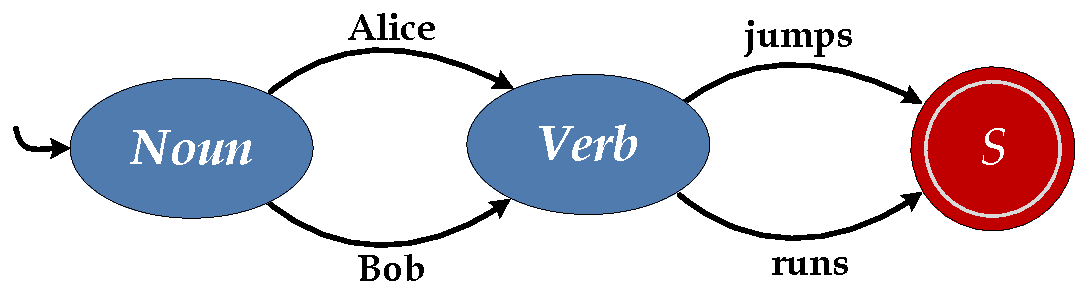
\includegraphics[height=0.85in]{figures/simple-rtn.pdf}
\caption{Simple recursive transition network.}\label{fig:simple-rtn}
\end{center}
\end{figure}

Recursive transition networks are more efficient than listing the strings in a language, since the number of possible strings increases with the number of possible paths through the graph.  For example, adding one more edge from \nonterminal{Noun} to \nonterminal{Verb} with label ``Colleen'' adds two new strings to the language.  

\index{general}{recursive definition}The expressive power of recursive transition networks increases dramatically once we add edges that form cycles in the graph.  This is where the \emph{recursive} in the name comes from. Once a graph has a cycle, there are \emph{infinitely} many possible paths through the graph!

Consider what happens when we add the single ``and'' edge to the previous network to produce the network shown in Figure~\ref{fig:cycle-rtn} below.

\begin{figure}[!ht]\centering
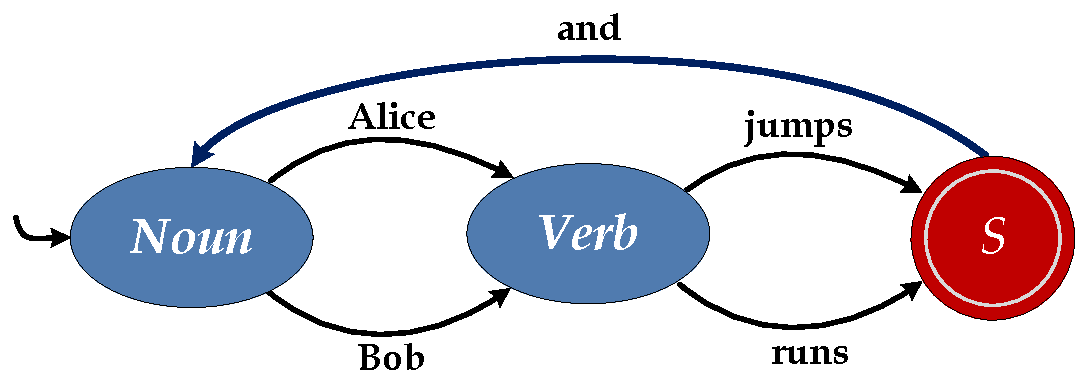
\includegraphics[height=1.2in]{figures/cycle-rtn.pdf}
\caption{RTN with a cycle.}\label{fig:cycle-rtn}
\end{figure}

Now, we can produce infinitely many different strings!  We can follow the ``and'' edge back to the \nonterminal{Noun} node to produce strings like ``Alice runs and Bob jumps and Alice jumps'' with as many conjuncts as we want.

\beforeex
\begin{exercise} \bluestar
Draw a recursive transition network that defines the language of the whole numbers: 0, 1, 2, $\ldots$
\solution{Since we expect a whole number to have at least one digit (the empty string is not allowed), and cannot have leading zeros (e.g., {\sf 003} is not a valid whole number), we need a special state to handle {\sf 0}.
\begin{center}
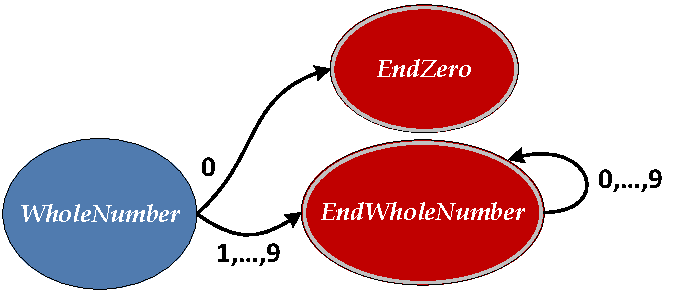
\includegraphics[height=1.25in]{figures/exercise-whole-numbers.pdf}
\end{center}
} 
\end{exercise}
\afterex

\beforeex
\begin{exercise}\label{exer:rtn-string}\bluestar How many different strings can be produced by the RTN below:
\begin{centernospace}
%\begin{figure}[!ht]\centering
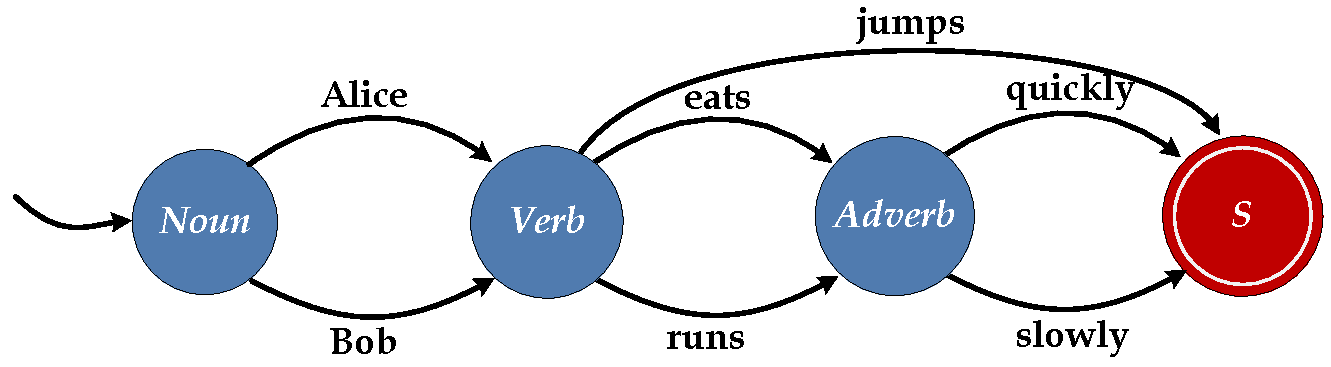
\includegraphics[height=1.3in]{figures/rtn-ex.pdf}
%\caption{RTN for Exercise~\ref{exer:rtn-string}.\label{fig:rtn-ex}}
%\end{figure}
\end{centernospace}
\solution{There are $10$ total strings, corresponding to each path through the RTN to the final \emph{S} state:
\emph{Alice jumps},
\emph{Alice eats slowly},
\emph{Alice eats quickly},
\emph{Alice runs slowly},
\emph{Alice runs quickly},
\emph{Bob jumps},
\emph{Bob eats slowly},
\emph{Bob eats quickly},
\emph{Bob runs slowly}
\emph{Bob runs quickly}.
}
\end{exercise}
\afterex

\beforesplitex
\begin{exercise} 
Recursive transition networks.
\begin{subexerciselist}
\item \bluestar How many nodes are needed for a recursive transition network that can produce exactly 8 strings? % 2 (for any number of strings)
\solution{Only 2 nodes are needed to produce any number of strings!  We can always have an arbitrary number of edges between the two nodes.
}
\item \greenstar How many edges are needed for a recursive transition network that can produce exactly 8 strings? % 2x2x2 = 6
\solution{If there is only one final state allowed, the minimum number of edges is 6.  To produce 8 total strings, we need two choices three times ($2 \times 2 \times 2 = 8$). 

\begin{center}
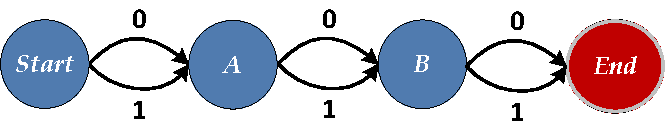
\includegraphics[width=4.5in]{figures/exercise-eight-strings.pdf}
\end{center}

If there can be more than one final state, though, it is possible to use only five edges!

\begin{center}
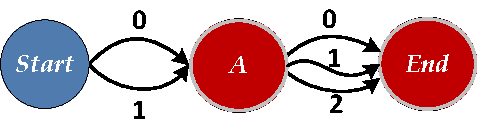
\includegraphics[width=3.2in]{figures/exercise-eight-strings-better.pdf}
\end{center}

I believe there is no RTN with fewer than five edges that can produce exactly 8 strings, but a convincing proof that this is the case is worth a gold star.
}


\item \doublegoldstar Given a whole number $n$, how many edges are needed for a recursive transition network that can produce exactly $n$ strings?
\solution{Unknown (at least to me)!  This is quite tricky, hence the \doublegoldstar.}
\end{subexerciselist}
\end{exercise}
\aftersplitex

\shortsection{Subnetworks}\label{sec:subnetworks}  In the RTNs we have seen so far, the labels on the output edges are direct outputs known as \emph{terminals}: following an edge just produces the symbol on that edge.  We can make more expressive RTNs by allowing edge labels to also name \emph{subnetworks}.  A subnetwork is identified by the name of its starting node.  When an edge labeled with a subnetwork is followed, the network traversal jumps to the subnetwork node.  Then, it can follow any path from that node to a final node.  Upon reaching a final node, the network traversal jumps back to complete the edge.  

For example, consider the network shown in Figure~\ref{fig:subnetwork-rtn}.  It describes the same language as the RTN in Figure~\ref{fig:simple-rtn}, but uses subnetworks for \nonterminal{Noun} and \nonterminal{Verb}.  To produce a string, we start in the \nonterminal{Sentence} node.  The only edge out from \nonterminal{Sentence} is labeled \nonterminal{Noun}.  To follow the edge, we jump to the \nonterminal{Noun} node, which is a separate subnetwork.  Now, we can follow any path from \nonterminal{Noun} to a final node (in this cases, outputting either ``Alice'' or ``Bob'' on the path toward \nonterminal{EndNoun}.  

\begin{figure}[!ht]
\centering
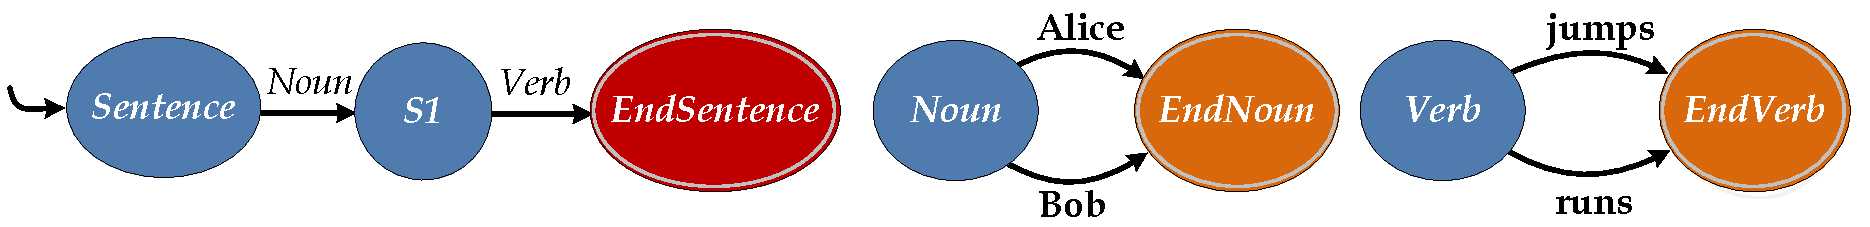
\includegraphics[width=4.75in]{figures/subnetwork-rtn.pdf}
\caption{Recursive transition network with subnetworks.}\label{fig:subnetwork-rtn}
\end{figure}

Suppose we replace the \nonterminal{Noun} subnetwork with the more interesting version shown in Figure~\ref{fig:andsubnetwork-rtn}.This subnetwork includes an edge from \nonterminal{Noun} to \nonterminal{N1} labeled \nonterminal{Noun}.  Following this edge involves following a path through the \nonterminal{Noun} subnetwork.  Starting from \nonterminal{Noun}, we can generate complex phrases like ``Alice and Bob'' or ``Alice and Bob and Alice'' (find the two different paths through the network that generate this phrase).

\begin{figure}[!hbt]
\centering
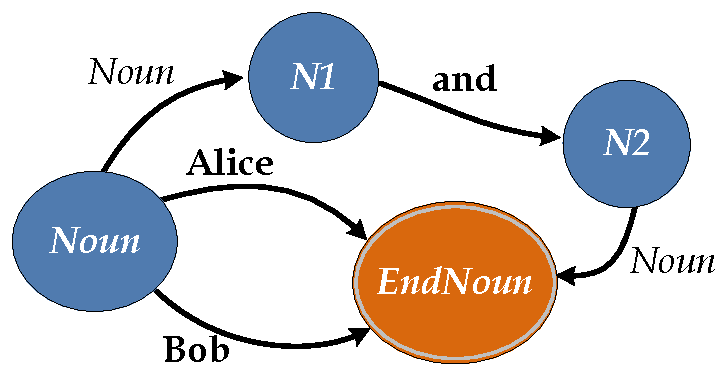
\includegraphics[height=1.2in]{figures/andsubnetwork-rtn.pdf}
\caption{Alternate \nonterminal{Noun} subnetwork.}\label{fig:andsubnetwork-rtn}
\end{figure}

To keep track of paths through RTNs without subnetworks, a single marker suffices.  We can start with the marker on the start node, and move it along the path through each node to the final node.  Keeping track of paths on an RTN with subnetworks is more complicated.  We need to keep track of where we are in the current network, and also where to continue to when a final node of the current subnetwork is reached.  Since we can enter subnetworks within subnetworks, we need a way to keep track of arbitrarily many jump points.

A \definition{stack} is a useful way to keep track of the subnetworks.  We can think of a stack like a stack of trays in a cafeteria.  At any point in time, only the top tray on the stack can be reached.  We can \emph{pop} the top tray off the stack, after which the next tray is now on top.  We can \emph{push} a new tray on top of the stack, which makes the old top of the stack now one below the top. 

We use a stack of nodes to keep track of the subnetworks as they are entered.  The top of the stack represents the next node to process.  At each step, we pop the node off the stack and follow a transition from that node.  

Using a stack, we can derive a path through an RTN using this procedure:
\begin{enumtight}
\item Initially, push the starting node on the stack.
\item If the stack is empty, {\bf stop}.  Otherwise, pop a node, $N$, off the stack.  
\item If the popped node, $N$, is a final node return to step 2.\footnote{For simplicity, this procedure assumes we always stop when a final node is reached.  RTNs can have edges out of final nodes (as in Figure~\ref{fig:cycle-rtn}) where it is possible to either stop or continue from a final node.}
\item Select an edge from the RTN that starts from node $N$.  Use $D$ to denote the destination of that edge, and $s$ to denote the output symbol on the edge.
\item Push $D$ on the stack. % step 5
\item If $s$ is a subnetwork, push the node $s$ on the stack.  Otherwise, output $s$, which is a terminal.
\item Go back to step 2. % step 7
\end{enumtight}

\begin{figure}[!t]\centering
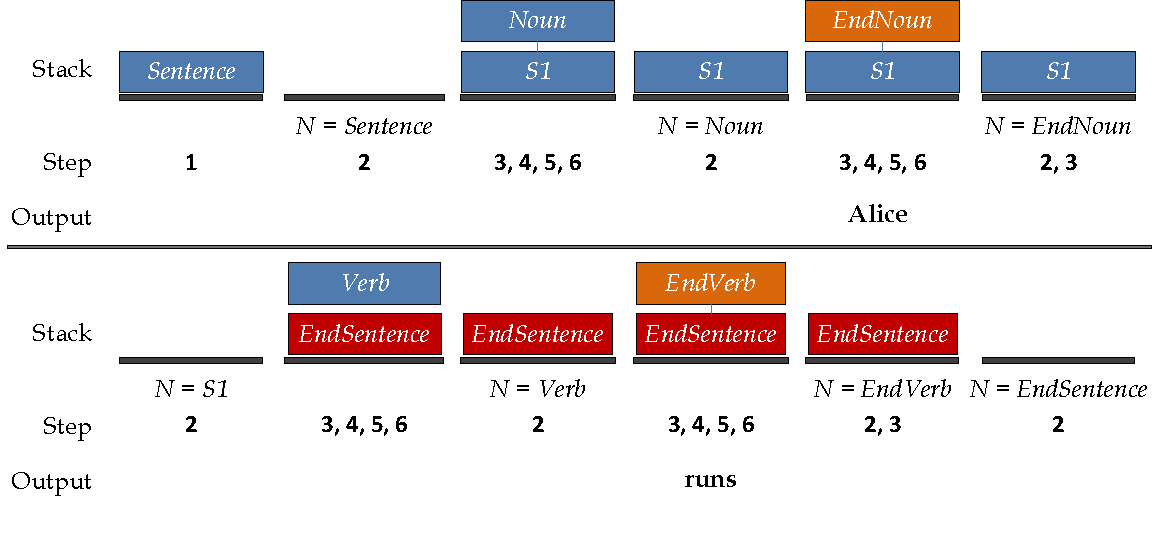
\includegraphics[width=4.85in]{figures/processing-rtn.pdf}
\caption{RTN generating ``Alice runs''.}\label{fig:rtn-processing}
\end{figure}

Consider generating the string ``Alice runs'' using the RTN in Figure~\ref{fig:subnetwork-rtn}.  We start following step 1 by pushing \nonterminal{Sentence} on the stack.  In step 2, we pop the stack, so the current node, $N$, is \nonterminal{Sentence}.  Since \nonterminal{Sentence} is not a final node, we do nothing for step 3.  In step 4, we follow an edge starting from \nonterminal{Sentence}.  There is only one edge to choose and it leads to the node labeled \nonterminal{S1}.  In step 5, we push \nonterminal{S1} on the stack.  The edge we followed is labeled with the node \nonterminal{Noun}, so we push \nonterminal{Noun} on the stack.  The stack now contains two items: $\left[\textsl{Noun}, \textsl{S1}\right]$. %$\left[\text{\nonterminal{Noun}}, \text{\nonterminal{S1}}\right]$.  
Since \nonterminal{Noun} is on top, this means we will first traverse the \nonterminal{Noun} subnetwork, and then continue from \nonterminal{S1}.

As directed by step 7, we go back to step 2 and continue by popping the top node, \nonterminal{Noun}, off the stack.  It is not a final node, so we continue to step 4, and select the edge labeled ``Alice'' from \nonterminal{Noun} to \nonterminal{EndNoun}.  We push \nonterminal{EndNoun} on the stack, which now contains: $\left[\textsl{EndNoun}, \textsl{S1}\right]$.  The label on the edge is the terminal, ``Alice'', so we output ``Alice'' following step 6.  We continue in the same manner, following the steps in the procedure as we keep track of a path through the network.  The full processing steps are shown in Figure~\ref{fig:rtn-processing}.

\beforeex
\begin{exercise}\bluestar 
Show the sequence of stacks used in generating the string ``Alice and Bob and Alice runs'' using the network in Figure~\ref{fig:subnetwork-rtn} with the alternate \nonterminal{Noun} subnetwork from Figure~\ref{fig:andsubnetwork-rtn}.
\solution{\LATER{}}
\end{exercise}
\afterex

\beforeex
\begin{exercise} \greenstar 
Identify a string that cannot be produced using the RTN from Figure~\ref{fig:subnetwork-rtn} with the alternate \nonterminal{Noun} subnetwork from Figure~\ref{fig:andsubnetwork-rtn} without the stack growing to contain five elements.
\solution{
For each \terminal{and}, the stack needs to grow to store either the \nonterminal{N1} or \nonterminal{N2} node (and one more node for the original \nonterminal{Noun}).
So, an example of a sentence that requires a stack depth of five is \terminal{Alice and Alice and Alice and Alice and Alice runs}.
}
\end{exercise}
\afterex

\beforeex
\begin{exercise} \bluestar 
The procedure given for traversing RTNs assumes that a subnetwork path always stops when a final node is reached.  Hence, it cannot follow all possible paths for an RTN where there are edges out of a final node.  Describe a procedure that can follow all possible paths, even for RTNs that include edges from final nodes.
\solution{To allow continuing from a final node, we need to change step 3 to be: If the popped node, $N$, is a final node either return to step 2 or continue to step 4.  Note that this procedure, as well as the original one, is \emph{nondeterministic}.  That means we cannot executed it by simply following the steps mechanically, but instead must make choices.  (In the original procedure, the choice was hidden in the \emph{Select} at the beginning of step 3 --- the procedure does not specify which edge to select when there are several choices.)  One way to mechanically execute a nondeterministic procedure is to systematically try all possible choices until one is found that leads to the desired solution (in this case, that is ending with an empty stack and the desired output).}
\end{exercise}
\afterex

\section{Replacement Grammars}\label{sec:grammars}

Another way to define a language is to use a grammar.\cut{\footnote{You are probably already somewhat familiar with grammars from your time in what was previously known as ``grammar school''!}}  This is the most common way languages are defined by computer scientists today, and the way we will use for the rest of this book.  

A \definition{grammar} is a set of rules for generating all strings in the language.  We use the {\em Backus-Naur Form} (BNF) notation to define a grammar.\index{general}{Backus-Naur Form}  BNF grammars are exactly as powerful as recursive transition networks (Exploration~\ref{exploration:power} explains what this means and why it is the case), but easier to write down.

BNF was invented by John Backus in the late 1950s.  
Backus led efforts at IBM to define and implement Fortran, the first widely used programming language.\index{general}{Fortran}\index{people}{Backus, John}  
Fortran enabled computer programs to be written in a language more like familiar algebraic formulas than low-level machine instructions, enabling programs to be written more quickly.  In defining the Fortran language, Backus and his team used ad hoc English descriptions to define the language.  
\sidepicture{0.20}{images/backus.jpg}{John Backus}{} % IBM image...permission needed? http://www.daylife.com/photo/0bwQ6Wiab45ut
These ad hoc descriptions were often misinterpreted, motivating the need for a more precise way of defining a language.  

\cut{Backus developed the replacement grammar notation to precisely describe the language of a later programming language, Algol (1958).  Peter Naur adapted the notation for the report describing the Algol language, and it was subsequently known as Backus-Naur Form at the suggestion of Donald Knuth to recognize both Backus' and Naur's contributions.}

Rules in a Backus-Naur Form grammar have the form:
\begin{bnfgrammarmc}{nonterminal}
\bnfrule{nonterminal}{\emph{replacement}}
\end{bnfgrammarmc}
\marginquote{I flunked out every year. I never studied. I hated studying. I was just goofing around. It had the delightful consequence that every year I went to summer school in New Hampshire where I spent the summer sailing and having a nice time.}{John Backus}
The left side of a rule is always a single symbol, known as a \emph{nonterminal} since it can never appear in the final generated string.  The right side of a rule contains one or more symbols.  
These symbols may include nonterminals, which will be replaced using replacement rules before generating the final string.  They may also be {\em terminals}, which are output symbols that never appear as the left side of a rule.  When we describe grammars, we use {\em italics} to represent nonterminal symbols, and \bold{bold} to represent terminal symbols.  The terminals are the primitives in the language; the grammar rules are its means of combination.

We can generate a string in the language described by a replacement grammar by starting from a designated start symbol (e.g., \nonterminal{sentence}), and at each step selecting a nonterminal in the working string, and replacing it with the right side of a replacement rule whose left side matches the nonterminal.  Wherever we find a nonterminal on the left side of a rule, we can replace it with what appears on the right side of any rule where that nonterminal matches the left side.  A string is generated once there are no nonterminals remaining.

Here is an example BNF grammar (that describes the same language as the RTN in Figure~\ref{fig:simple-rtn}):
\begin{bnfgrammarmn}{Sentence}
\bnfrulen{1}{Sentence}{\nonterminal{Noun} \nonterminal{Verb}}
\bnfrulen{2}{Noun}{\terminal{Alice}}
\bnfrulen{3}{Noun}{\terminal{Bob}}
\bnfrulen{4}{Verb}{\terminal{jumps}}
\bnfrulen{5}{Verb}{\terminal{runs}}
\end{bnfgrammarmn}
Starting from \nonterminal{Sentence}, the grammar can generate four sentences: ``Alice jumps'', ``Alice runs'', ``Bob jumps'', and ``Bob runs''.  

A \definition{derivation} shows how a grammar generates a given string.  Here is the derivation of ``Alice runs'':
\begin{smallquote}
\begin{tabbing}
\nonterminal{Sentence} \= \produces \= \nonterminal{\underline{Noun}} \nonterminal{Verb}\hspace*{6em}\=using Rule 1\\
\> \produces \= {\bf Alice} \nonterminal{\underline{Verb}} \> replacing \nonterminal{Noun} using Rule 2\\
\> \produces \= {\bf Alice} {\bf runs} \>	replacing \nonterminal{Verb} using Rule 5\\
\end{tabbing}
\end{smallquote}
We can represent a grammar derivation as a tree, where the root of the tree is the starting nonterminal (\nonterminal{Sentence} in this case), and the leaves of the tree are the terminals that form the derived sentence.  Such a tree is known as a \definition{parse tree}.  Here is the parse tree for the derivation of ``Alice runs'':
\begin{center}
\Treek{1.5}{ & \K{\nonterminal{Sentence}} \B{dl} \B{dr} \\
       \K{\nonterminal{Noun}} \B{d} & & \K{\nonterminal{Verb}} \B{d} \\
       \K{{\bf Alice}} & & \K{{\bf runs}}}
\end{center}
BNF grammars can be more compact than just listing strings in the language since a grammar can have many replacements for each nonterminal.  For example, adding the rule, \bnfshowrule{Noun}{\terminal{Colleen}}, to the grammar adds two new strings (``Colleen runs'' and ``Colleen jumps'') to the language.  

\shortsection{Recursive Grammars}\index{general}{recursive grammar}The real power of BNF as a compact notation for describing languages, though, comes once we start adding recursive rules to our grammar.   A grammar is recursive if the grammar contains a nonterminal that can produce a production that contains itself.  

Suppose we add the rule, 
\begin{centernospace}
\bnfshowrule{Sentence}{\nonterminal{Sentence} \terminal{and} \nonterminal{Sentence}}
\end{centernospace}
%\begin{bnfgrammarmn}{Sentence}
%\bnfrulen{6}{Sentence}{\nonterminal{Sentence} \terminal{and} \nonterminal{Sentence}}
%\end{bnfgrammarmn}
to our example grammar.  Now, how many sentences can we generate?

Infinitely many!  This grammar describes the same language as the RTN in Figure~\ref{fig:cycle-rtn}.  It can generate ``Alice runs and Bob jumps'' and ``Alice runs and Bob jumps and Alice runs'' and sentences with any number of repetitions of ``Alice runs''.  This is very powerful: by using recursive rules a compact grammar can be used to define a language containing infinitely many strings.

\clearpage %!!
\begin{examplenobar}{Whole Numbers}\label{example:wholenumbers} This grammar defines the language of the whole numbers (0, 1, $\ldots$) with leading zeros allowed:
\vspace*{6pt}

\begin{minipage}[b]{0.5\linewidth}
\begin{bnfgrammarm}{MoreDigits}
\bnfrule{Number}{\nonterminal{Digit} \nonterminal{MoreDigits}}
\bnfrule{MoreDigits}{}
\bnfrule{MoreDigits}{\nonterminal{Number}}
\bnfrule{Digit}{\terminal{0}}
\bnfrule{Digit}{\terminal{1}}
\bnfrule{Digit}{\terminal{2}}
\bnfrule{Digit}{\terminal{3}}
\end{bnfgrammarm}
\end{minipage}
\begin{minipage}[b]{0.4\linewidth}
\begin{bnfgrammarm}{Digit}
\bnfrule{Digit}{\terminal{4}}
\bnfrule{Digit}{\terminal{5}}
\bnfrule{Digit}{\terminal{6}}
\bnfrule{Digit}{\terminal{7}}
\bnfrule{Digit}{\terminal{8}}
\bnfrule{Digit}{\terminal{9}}
\end{bnfgrammarm}
\end{minipage}

Here is the parse tree for a derivation of {\bf 37} from \nonterminal{Number}:
\begin{centernospace}
\Treek{1.4}{ &      \K{\nonterminal{Number}} \B{dl} \B{dr} \\
       \K{\nonterminal{Digit}} \B{d} & & \K{\nonterminal{MoreDigits}} \B{d}  \\
       \K{{\bf 3}}            & & \K{\nonterminal{Number}} \B{dl} \B{dr} \\
       &              \K{\nonterminal{Digit}} \B{d} & & \K{\nonterminal{MoreDigits}} \B{d} \\
       &              \K{\bf 7}              & & \K{$\epsilon$}} 
\end{centernospace}
\shortsection{Circular vs. Recursive Definitions}  The second rule means we can replace \nonterminal{MoreDigits} with nothing.  This is sometimes written as $\epsilon$ to make it clear that the replacement is empty: \bnfshowrule{MoreDigits}{$\epsilon$}.
%\begin{bnfgrammarm}{MoreDigits}
%\bnfrule{MoreDigits}{$\epsilon$}
%\end{bnfgrammarm}

This is a very important rule in the grammar---without it \emph{no} strings could be generated; with it \emph{infinitely} many strings can be generated.  The key is that we can only produce a string when all nonterminals in the string have been replaced with terminals.  Without the \bnfshowrule{MoreDigits}{$\epsilon$} rule, the only rule we would have with \nonterminal{MoreDigits} on the left side is the third rule: \bnfshowrule{MoreDigits}{\nonterminal{Number}}.
%\begin{bnfgrammarm}{MoreDigits}
%\bnfrule{MoreDigits}{\nonterminal{Number}}
%\end{bnfgrammarm}

The only rule we have with \nonterminal{Number} on the left side is the first rule, which replaces \nonterminal{Number} with \nonterminal{Digit} \nonterminal{MoreDigits}.  Every time we follow this rule, we replace \nonterminal{MoreDigits} with \nonterminal{Digit} \nonterminal{MoreDigits}.  We can produce as many \nonterminal{Digit}s as we want, but without the \bnfshowrule{MoreDigits}{$\epsilon$} rule we can never stop.  

This is the difference between a \emph{circular} definition, and a \emph{recursive} definition.  Without the stopping rule, \nonterminal{MoreDigits} would be defined in a circular way.  There is no way to start with \nonterminal{MoreDigits} and generate a production that does not contain \nonterminal{MoreDigits} (or a nonterminal that eventually must produce \nonterminal{MoreDigits}).  With the \bnfshowrule{MoreDigits}{$\epsilon$} rule, however, we have a way to produce something terminal from \nonterminal{MoreDigits}.  This is known as a \definition{base case} --- a rule that turns an otherwise circular definition into a meaningful, recursive definition.  

\shortsection{Condensed Notation}
It is common to have many grammar rules with the same left side nonterminal.  For example, the whole numbers grammar has ten rules with \nonterminal{Digit} on the left side to produce the ten terminal digits.  Each of these is an alternative rule that can be used when the production string contains the nonterminal \nonterminal{Digit}.  A compact notation for these types of rules is to use the vertical bar ($\mid$) to separate alternative replacements.  For example, we could write the ten \nonterminal{Digit} rules compactly as:
\begin{bnfgrammarm}{Digit}
\bnfrule{Digit}{\terminal{0} $\mid$ \terminal{1} $\mid$ \terminal{2} $\mid$ \terminal{3} $\mid$ \terminal{4} $\mid$ \terminal{5} $\mid$ \terminal{6} $\mid$ \terminal{7} $\mid$ \terminal{8} $\mid$ \terminal{9}}
\end{bnfgrammarm} 
%This means exactly the same thing as listing the ten digit rules separately as in the original example.

\beforeex
\begin{exercise}
Suppose we replaced the first rule (\bnfshowrule{Number}{\nonterminal{Digit} \nonterminal{MoreDigits}}) in the whole numbers grammar with: \bnfshowrule{Number}{\nonterminal{MoreDigits} \nonterminal{Digit}}. 
\begin{subexerciselist}
\item \bluestar How does this change the parse tree for the derivation of {\bf 37}?  Draw the parse tree that results from the new grammar.
\solution{
\begin{centernospace}
\Treek{1.4}{ &      &                  \K{\nonterminal{Number}} \B{dl} \B{dr}  \\
             &      \K{\nonterminal{MoreDigits}} \B{d}    &  &  \K{\nonterminal{Digit}} \B{d}  \\
             &      \K{\nonterminal{Number}} \B{dl}\B{dr} &  &  \K{{\bf 7}} \\
             \K{\nonterminal{Digit}} \B{d} & & \K{\nonterminal{MoreDigits}} \B{d} \\
             \K{\bf 3}                     & & \K{$\epsilon$}  \\
       }
\end{centernospace}
}


\item \greenstar Does this change the language?  Either show some string that is in the language defined by the modified grammar but not in the original language (or vice versa), or argue that both grammars generate the same strings.
\solution{
Although this changes the way numbers are parsed, it does not change the language.  The production \bnfshowrule{Number}{\nonterminal{Digit} \nonterminal{MoreDigits}}
generates the same strings as  \bnfshowrule{Number}{\nonterminal{MoreDigits} \nonterminal{Digit}} since \nonterminal{MoreDigits} is the same in both, and it generates a sequence of zero or more digits.  The difference is whether the single digit produced by \nonterminal{Digit} is before or after the sequence of zero or more digits produces by \nonterminal{MoreDigits}.  Since all digits are interchangeable, though, this produces the same set of strings. 
}
\end{subexerciselist}
\end{exercise}
\afterex

\beforeex
\begin{exercise} \bluestar
The grammar for whole numbers we defined allows strings with non-standard leading zeros such as ``000'' and ``00005''.  Devise a grammar that produces all whole numbers (including ``0''), but no strings with unnecessary leading zeros.
\solution{
To eliminate the leading zeros, we need to add a new nonterminal for \nonterminal{NonZeroDigit}, and a special rule for \terminal{0}.
\begin{bnfgrammarm}{NonZeroDigit}
\bnfrule{Number}{\terminal{0}}
\bnfrule{Number}{\nonterminal{NonZeroDigit} \nonterminal{MoreDigits}}
\bnfrule{MoreDigits}{}
\bnfrule{MoreDigits}{\nonterminal{Digit} \nonterminal{MoreDigits}}
\bnfrule{Digit}{\terminal{0}}
\bnfrule{Digit}{\nonterminal{NonZeroDigit}}
\bnfrule{NonZeroDigit}{\terminal{1} $\mid$ \terminal{2} $\mid$ $\cdots$ $\mid$ \terminal{9}}
\end{bnfgrammarm}
}

\end{exercise}
\afterex

\beforeex
\begin{exercise} \greenstar 
Define a BNF grammar that describes the language of decimal numbers (the language should include 3.14159, 0.423, and 1120 but not 1.2.3).
\solution{
We assume the \nonterminal{Number} definition from Example~\ref{example:wholenumbers}.
\begin{bnfgrammarm}{OptMantissa}
\bnfrule{Decimal}{\nonterminal{Number} \nonterminal{OptMantissa}}
\bnfrule{OptMantissa}{$\epsilon$}
\bnfrule{OptMantissa}{\terminal{.} \nonterminal{Number}}
\end{bnfgrammarm}
This does allow numbers like \terminal{003.200}.  A stricter definition of decimal numbers that disallows leading zeros would use the \nonterminal{Number} definition from the previous exercise, but would need to define a \nonterminal{FullNumber} nonterminal also to allow leading zeros to the right of the decimal point.
}
\end{exercise}
\afterex

\end{examplenobar}

\cut{\ex{\bluestar
The grammar for whole numbers is complicated because we do not want to include the empty string in our language.  Devise a simpler grammar that defines the language of the whole numbers including the empty string.}
}

\index{general}{domain names}\index{people}{Mockapetrics, Paul}
\beforesplitex
\begin{exercise} \greenstar \label{exercise:domains}
The BNF grammar below (extracted from Paul Mockapetris, \emph{Domain Names - Implementation and Specification}, IETF RFC 1035) describes the language of domain names on the Internet.

\begin{bnfgrammarm}{SubDomainList}
\bnfrule{Domain}{\nonterminal{SubDomainList}}
\bnfrule{SubDomainList}{\nonterminal{Label} $\mid$ \nonterminal{SubDomainList} \terminal{.} \nonterminal{Label}}
\bnfrule{Label}{\nonterminal{Letter} \nonterminal{MoreLetters}}
\bnfrule{MoreLetters}{\nonterminal{LetterHyphens} \nonterminal{LetterDigit} $\mid$ $\epsilon$}
\bnfrule{LetterHyphens}{\nonterminal{LDHyphen} $\mid$ \nonterminal{LDHyphen} \nonterminal{LetterHyphens} $\mid$ $\epsilon$}
\bnfrule{LDHyphen}{\nonterminal{LetterDigit} $\mid$ \terminal{-}}
\bnfrule{LetterDigit}{\nonterminal{Letter} $\mid$ \nonterminal{Digit}}
\bnfrule{Letter}{\terminal{A} $\mid$ \terminal{B} $\mid$ $\ldots$ $\mid$ \terminal{Z} $\mid$ \terminal{a} $\mid$ \terminal{b} $\mid$ $\ldots$ $\mid$ \terminal{z}}
\bnfrule{Digit}{\terminal{0} $\mid$ \terminal{1} $\mid$ \terminal{2} $\mid$ \terminal{3} $\mid$ \terminal{4} $\mid$ \terminal{5} $\mid$ \terminal{6} $\mid$ \terminal{7} $\mid$ \terminal{8} $\mid$ \terminal{9}}
\end{bnfgrammarm}
\begin{subexerciselist}
\item Show a derivation for \terminal{www.virginia.edu} in the grammar.
\solution{
Note that the grammar is ambiguous, so there are many other ways to produce the same string.  Here is one possible derivation: 
\begin{smallquote}
\begin{tabbing}
\nonterminal{Domain} \= \produces\quad \= \nonterminal{\underline{SubDomainList}} \hspace*{6em}\=\\
                     \> \produces \> \nonterminal{SubDomainList} {\bf .} \nonterminal{\underline{Label}} \> \\
                     \> \produces \> \nonterminal{SubDomainList} {\bf .} \nonterminal{\underline{Letter}} \nonterminal{MoreLetters} \> \\
                     \> \produces \> \nonterminal{SubDomainList} {\bf .} {\bf e} \nonterminal{\underline{MoreLetters}} \> \\
                     \> \produces \> \nonterminal{SubDomainList} {\bf .} {\bf e} \nonterminal{\underline{LetterHyphens}} \nonterminal{LetterDigit} \> \\
                     \> \produces \> \nonterminal{SubDomainList} {\bf .} {\bf e} \nonterminal{\underline{LDHyphen}} \nonterminal{LetterHyphens} \nonterminal{LetterDigit} \> \\
                     \> \produces \> \nonterminal{SubDomainList} {\bf .} {\bf e} \nonterminal{\underline{LetterDigit}} \nonterminal{LetterHyphens} \nonterminal{LetterDigit} \> \\
                     
                     \> \produces \> \nonterminal{SubDomainList} {\bf .} {\bf e} \nonterminal{\underline{Letter}} \nonterminal{LetterHyphens} \nonterminal{LetterDigit} \> \\

                     \> \produces \> \nonterminal{SubDomainList} {\bf .} {\bf e} {\bf d} \nonterminal{\underline{LetterHyphens}} \nonterminal{LetterDigit} \> \\
                     \> \produces \> \nonterminal{SubDomainList} {\bf .} {\bf e} {\bf d} \nonterminal{\underline{LetterDigit}} \hspace*{2em} (using \nonterminal{LetterHyphens} \produces $\epsilon$)\\
                     \> \produces \> \nonterminal{SubDomainList} {\bf .} {\bf e} {\bf d} \nonterminal{\underline{Letter}} \> \\
                     \> \produces \> \nonterminal{\underline{SubDomainList}} {\bf .} {\bf e} {\bf d} {\bf u} \> \\
                     \> \produces$^*$ \> \nonterminal{SubDomainList} {\bf .} \nonterminal{\underline{Label}} {\bf .} {\bf e} {\bf d} {\bf u} \hspace*{2em} (we fast-forward the steps for \nonterminal{Label} \produces$^*$ {\bf virginia}) \\ 
                     \> \produces \> \nonterminal{\underline{SubDomainList}} {\bf .} {\bf v} {\bf i} {\bf r} {\bf g} {\bf i} {\bf n} {\bf i} {\bf a} {\bf .} {\bf e} {\bf d} {\bf u} \> \\
                     \> \produces \> \nonterminal{\underline{Label}} {\bf .} {\bf v} {\bf i} {\bf r} {\bf g} {\bf i} {\bf n} {\bf i} {\bf a} {\bf .} {\bf e} {\bf d} {\bf u} \> \\
                     \> \produces \> {\bf w} {\bf w} {\bf w} {\bf .} {\bf v} {\bf i} {\bf r} {\bf g} {\bf i} {\bf n} {\bf i} {\bf a} {\bf .} {\bf e} {\bf d} {\bf u} \hspace{2em} (fast-forwarding \nonterminal{Label} \produces$^*$ {\bf w} {\bf w} {\bf w}) \\
\end{tabbing}
\end{smallquote}
}
\item According to the grammar, which of the following are valid domain names: (1) \terminal{tj}, (2) \terminal{a.-b.c}, (3) \terminal{a-a.b-b.c-c}, (4) \terminal{a.g.r.e.a.t.d.o.m.a.i.n-}.
\solution{
\begin{description}
\item (1) \terminal{tj} is a grammatically valid domain name: \nonterminal{Domain} \produces \nonterminal{SubDomainList} \produces \nonterminal{Label} \produces$^*$ \terminal{tj}.

\item (2) \terminal{a.-b.c} is not a grammatically valid domain name.  The \nonterminal{Label} cannot produce the string \terminal{-b} since the only production for \nonterminal{Label} is \nonterminal{Label} \produces \nonterminal{Letter} \nonterminal{MoreLetters} and \nonterminal{Letter} cannot produce \terminal{-}.

\item (3) \terminal{a-a.b-b.c-c} is a grammatically valid domain name: 
\nonterminal{Domain} \produces \nonterminal{SubDomainList} \produces$^*$ \nonterminal{Label} \terminal{.} \nonterminal{Label} \terminal{.} \nonterminal{Label} \produces$^*$ \terminal{a-a.b-b.c-c}.

\item (4) \terminal{a.g.r.e.a.t.d.o.m.a.i.n-} is a not grammatically valid domain name.  The \nonterminal{Label} productions cannot produce a label that ends in a \terminal{-} since \nonterminal{MoreLetters} \produces \nonterminal{LetterHyphens} \nonterminal{LetterDigit} $\mid$ $\epsilon$ a label must end in a letter or digit.  
\end{description}
}

\end{subexerciselist}
\end{exercise}
\aftersplitex

\cut{
\ex{\doublegoldstar
Devise a grammar that defines the language of valid dates (e.g., ``December 7, 1941'').  Your language should include all valid dates, but no invalid dates (that is, ``September 29, 2007'' and ``February 29, 2008'' are in the language, but ``February 29, 2009'' is not).
}
}

%!\clearpage %!!!
\splitexplorenobar{Power of Language Systems}{
\label{exploration:power}
Section~\ref{sec:grammars} claimed that recursive transition networks and BNF grammars are equally powerful.  What does it mean to say two systems are equally powerful? 

A language description mechanism is used to define a set of strings comprising a language.  Hence, the power of a language description mechanism is determined by the set of languages it can define.  

One approach to measure the power of language description mechanism would be to count the number of languages that it can define.  Even the simplest mechanisms can define infinitely many languages, however, so just counting the number of languages does not distinguish well between the different language description mechanisms.  Both RTNs and BNFs can describe infinitely many different languages.  We can always add a new edge to an RTN to increase the number of strings in the language, or add a new replacement rule to a BNF that replaces a nonterminal with a new terminal symbol.

Instead, we need to consider the set of languages that each mechanism can define.  A system $A$ is more powerful that another system $B$ if we can use $A$ to define every language that can be defined by $B$, and there is some language $L$ that can be defined using $A$ that cannot be defined using $B$.  This matches our intuitive interpretation of \emph{more powerful} --- $A$ is more powerful than $B$ if it can do everything $B$ can do and more.  

The diagrams in Figure~\ref{fig:language-power} show three possible scenarios.  In the leftmost picture, the set of languages that can be defined by $B$ is a proper subset of the set of languages that can be defined by $A$.  Hence, $A$ is more powerful than $B$.  In the center picture, the sets are equal.  This means every language that can be defined by $A$ can also be defined by $B$, and every language that can be defined by $B$ can also be defined by $A$, and the systems are equally powerful.  In the rightmost picture, there are some elements of $A$ that are not elements of $B$, but there are also some elements of $B$ that are not elements of $A$.  This means we cannot say either one is more powerful; $A$ can do some things $B$ cannot do, and $B$ can do some things $A$ cannot do.

\begin{figure}[bth]\centering
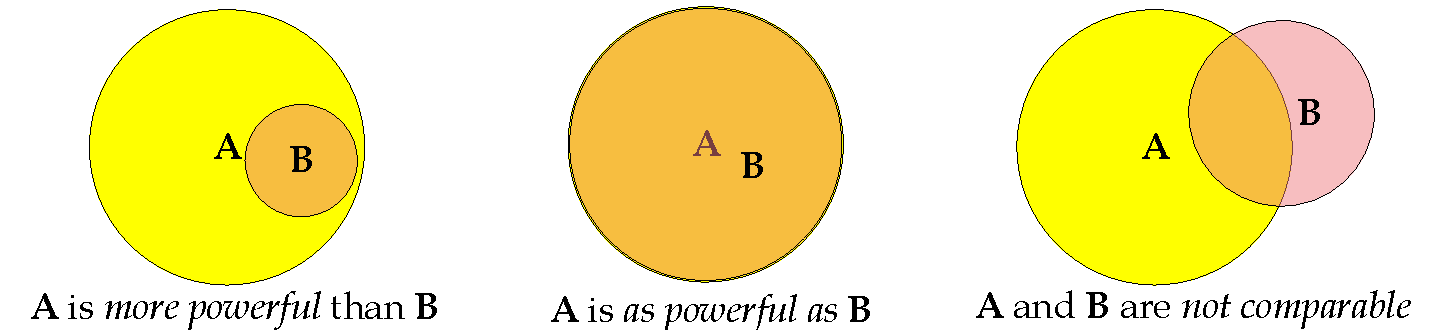
\includegraphics[width=5.0in]{figures/language-power.pdf}
\caption{System power relationships.}\label{fig:language-power}
\end{figure}
To determine the relationship between RTNs and BNFs we need to understand if there are languages that can be defined by a BNF that cannot be defined by a RTN and if there are languages that can be defined by a RTN that cannot be defined by an BNF.  We will show only the first part of the proof here, and leave the second part as an exercise.

For the first part, we prove that there are no languages that can be defined by a BNF that cannot be defined by an RTN.  Equivalently, \emph{every} language that can be defined by a BNF grammar has a corresponding RTN.  Since there are infinitely many languages that can be defined by BNF grammars, we cannot prove this by enumerating each language and showing its corresponding RTN.  Instead, we use a proof technique commonly used in computer science: \definition{proof by construction}.  We show an algorithm that given any BNF grammar constructs an RTN that defines the same language as the input BNF grammar.  

Our strategy is to construct a subnetwork corresponding to each nonterminal.  For each rule where the nonterminal is on the left side, the right hand side is converted to a path through that node's subnetwork.  

Before presenting the general construction algorithm, we illustrate the approach with the example BNF grammar from Example~\ref{example:wholenumbers}:

\begin{bnfgrammarm}{MoreDigits}
\bnfrule{Number}{\nonterminal{Digit} \nonterminal{MoreDigits}}
\bnfrule{MoreDigits}{$\epsilon$}
\bnfrule{MoreDigits}{\nonterminal{Number}}
\bnfrule{Digit}{\terminal{0} $\mid$ \terminal{1} $\mid$ \terminal{2} $\mid$ \terminal{3} $\mid$ \terminal{4} $\mid$ \terminal{5} $\mid$ \terminal{6} $\mid$ \terminal{7} $\mid$ \terminal{8} $\mid$ \terminal{9}}
\end{bnfgrammarm}

The grammar has three nonterminals: \nonterminal{Number}, \nonterminal{Digit}, and \nonterminal{MoreDigits}.  For each nonterminal, we construct a subnetwork by first creating two nodes corresponding to the start and end of the subnetwork for the nonterminal.  We make \nonterminal{StartNumber} the start node for the RTN since \nonterminal{Number} is the starting nonterminal for the grammar.  

Next, we need to add edges to the RTN corresponding to the production rules in the grammar.  The first rule indicates that \nonterminal{Number} can be replaced by \nonterminal{Digit} \nonterminal{MoreDigits}.  To make the corresponding RTN, we need to introduce an intermediate node since each RTN edge can only contain one label.  We need to traverse two edges, with labels \nonterminal{StartDigit} and \nonterminal{StartMoreDigits} between the \nonterminal{StartNumber} and \nonterminal{EndNumber} nodes.  The resulting partial RTN is shown in Figure~\ref{fig:convert-number}.

\begin{figure}[htbp]
\begin{center}
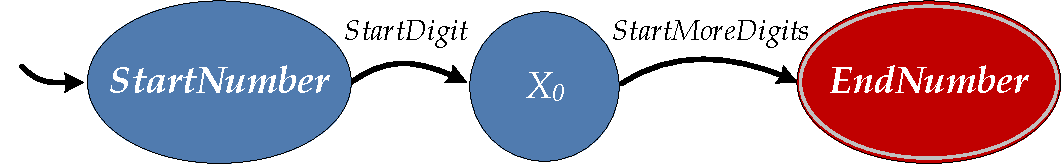
\includegraphics[width=4.5in]{figures/convert-rtn-number.pdf}
\end{center}
\caption{Converting the \nonterminal{Number} productions to an RTN.\label{fig:convert-number}}
\end{figure}

For the \nonterminal{MoreDigits} nonterminal there are two productions.  The first means \nonterminal{MoreDigits} can be replaced with nothing.  In an RTN, we cannot have edges with unlabeled outputs.  So, the equivalent of outputting nothing is to turn \nonterminal{StartMoreDigits} into a final node.  The second production replaces \nonterminal{MoreDigits} with \nonterminal{Number}.  We do this in the RTN by adding an edge between \nonterminal{StartMoreDigits} and \nonterminal{EndMoreDigits} labeled with \nonterminal{Number}, as shown in Figure~\ref{fig:convert-moredigits}.

\begin{figure}[!htbp]
\begin{center}

\includegraphics[height=0.6in]{figures/convert-rtn-moredigits.pdf}
\end{center}
\caption{Converting the \nonterminal{MoreDigits} productions to an RTN.}\label{fig:convert-moredigits}
\end{figure}

Finally, we convert the ten \nonterminal{Digit} productions.  For each rule, we add an edge between \nonterminal{StartDigit} and \nonterminal{EndDigit} labeled with the digit terminal, as shown in Figure~\ref{fig:convert-digit}.

\begin{figure}[!htbp]
\begin{center}

\includegraphics[height=0.75in]{figures/convert-rtn-digit.pdf}
\end{center}
\caption{Converting the \nonterminal{Digit} productions to an RTN.}\label{fig:convert-digit}
\end{figure}

This example illustrates that it is possible to convert a particular grammar to an RTN.  For a general proof, we present a general an algorithm that can be used to do the same conversion for any BNF:

\begin{enumerate}
\item For each nonterminal \emph{X} in the grammar, construct two nodes, \nonterminal{Start}\emph{X} and \nonterminal{End}\emph{X}, where \nonterminal{End}\emph{X} is a final node.  Make the node \nonterminal{Start}\emph{S} the start node of the RTN, where \emph{S} is the start nonterminal of the grammar.
\item For each rule in the grammar, add a corresponding path through the RTN.  All BNF rules have the form \bnfshowrule{\emph{X}}{\emph{replacement}} where \emph{X} is a nonterminal in the grammar and \emph{replacement} is a sequence of zero or more terminals and nonterminals: $\left[ R_0, R_1, \ldots, R_n \right]$.  
\begin{enumerate}
\item If the replacement is empty, make \nonterminal{Start}\emph{X} a final node.
\item If the replacement has just one element, $R_0$, add an edge from \nonterminal{Start}\emph{X} to \nonterminal{End}\emph{X} with edge label $R_0$. 
\item Otherwise:
\begin{enumerate}
\item Add an edge from \nonterminal{Start}\emph{X} to a new node labeled $X_{i,0}$ (where $i$ identifies the grammar rule), with edge label $R_0$.
\item For each remaining element $R_j$ in the replacement add an edge from $X_{i,j-1}$ to a new node labeled $X_{i,j}$ with edge label $R_j$.  (For example, for element $R_1$, a new node $X_{i,1}$ is added, and an edge from $X_{i,0}$ to $X_{i,1}$ with edge label $R_1$.)
\item Add an edge from $X_{i,n-1}$ to \nonterminal{End}\emph{X} with edge label $R_n$.
\end{enumerate}
\end{enumerate}
\end{enumerate}

Following this procedure, we can convert any BNF grammar into an RTN that defines the same language.  Hence, we have proved that RTNs are at least as powerful as BNF grammars.

To complete the proof that BNF grammars and RTNs are equally powerful ways of defining languages, we also need to show that a BNF can define every language that can be defined using an RTN.  This part of the proof can be done using a similar strategy in reverse: by showing a procedure that can be used to construct a BNF equivalent to any input RTN.  We leave the details as an exercise for especially ambitious readers.
}

\beforeex
\begin{exercise} \greenstar 
Produce an RTN that defines the same languages as the BNF grammar from Exercise~\ref{exercise:domains}.
\solution{
\begin{center}
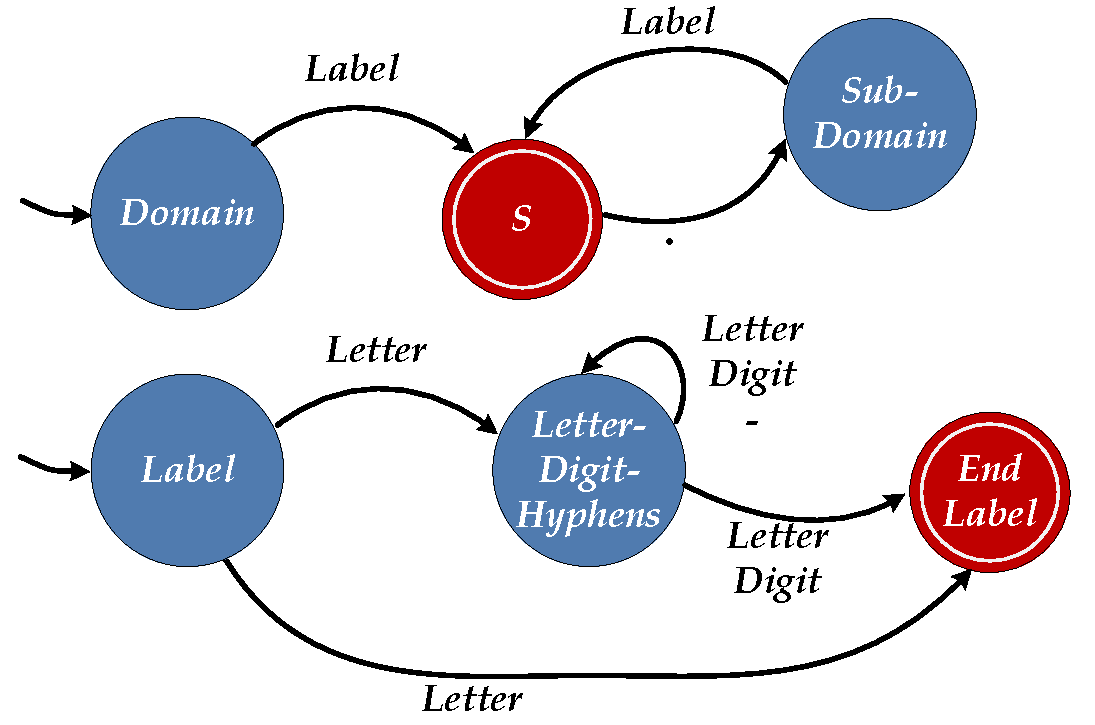
\includegraphics[width=5.0in]{figures/rtn-domains.pdf}
\end{center}
Note the need for the bottom edge from \nonterminal{Label} to \nonterminal{EndLabel} that is necessary to allow single-letter labels.
}
\end{exercise}
\afterex

\beforeex
\begin{exercise} \goldstar
Prove that BNF grammars are as powerful as RTNs by devising a procedure that can construct a BNF grammar that defines the same language as any input RTN.
\solution{\LATER{}}
\end{exercise}
\afterex

\section{Summary}

Languages define a set of surface forms and associated meanings.  Since useful language must be able to express infinitely many things, we need tools for defining infinite sets of surface forms using compact and precise notations.  The tool we will use for the remainder of this book is the BNF replacement grammar which precisely defines a language using replacement rules.  This system can describe infinite languages with small representations because of the power of recursive rules.  In the next chapter, we introduce the Scheme programming language that we will use to describe procedures. 

\begin{comment}
further reading:

books about language:
	pinker, yang

John Backus and Fortran?

Post

\end{comment}
